\documentclass[11pt]{article}
\usepackage{amsmath}
\usepackage{tikz}
\usepackage{amsmath}
\usetikzlibrary{automata,positioning}
\usepackage{tikz}
\DeclareRobustCommand{\orcidicon}{
	
\begin{tikzpicture}
	\draw[lime, fill=lime] (0,0) 
	circle [radius=0.16] 
	node[white] {{\fontfamily{qag}\selectfont \tiny ID}};
	\draw[white, fill=white] (-0.0625,0.095) 
	circle [radius=0.007];
	\end{tikzpicture}
	\hspace{-2mm}
}
\usepackage{xcolor}

\begin{document}

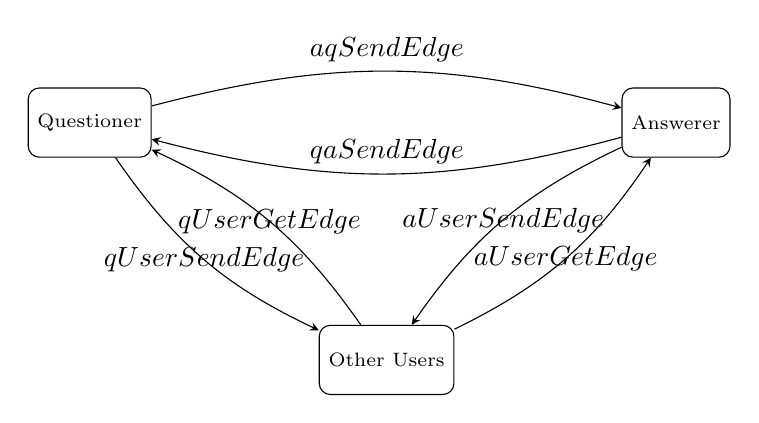
\begin{tikzpicture}[>=stealth, node distance=3cm, state/.append style={font=\scriptsize, shape=rectangle, rounded corners, top color=white}] 
	 
            \node[state] (A2) {Questioner};
            \node[state,below right=of A2] (C2) {Other Users};
            \node[state,above right=of C2] (B2) {Answerer};
           
            \draw (A2) edge[->,bend left=15, above] node {$aqSendEdge$} (B2);
            \draw (B2) edge[->,bend left=15, above] node {$qaSendEdge$} (A2);
            
            \draw (C2) edge[<-,bend left=15] node {$qUserSendEdge$} (A2);
            \draw (A2) edge[<-,bend left=15] node {$qUserGetEdge$} (C2);
            
            \draw (C2) edge[<-,bend left=15] node {$aUserSendEdge$} (B2);
            \draw (B2) edge[<-,bend left=15] node {$aUserGetEdge$} (C2);

	\end{tikzpicture}

\end{document}